% You should title the file with a .tex extension (hw1.tex, for example)
\documentclass[11pt]{article}

\usepackage{amsmath}
\usepackage{amssymb}
\usepackage{fancyhdr}
\usepackage{graphicx}
\usepackage{listings}

\oddsidemargin0cm
\topmargin-1.7cm     %I recommend adding these three lines to increase the 
\textwidth16.5cm   %amount of usable space on the page (and save trees)
\textheight23.5cm  

\parskip = 1em % add some space between paragraphs

\pagestyle{fancyplain}
\lhead{\fancyplain{}{11-411 Natural Language Processing}}      % Note the different brackets!
\rhead{\fancyplain{}{Broccoli}}
\chead{\fancyplain{}{Project Report}}
\begin{document}
  
  \thispagestyle{plain}
  \title{11-411 Final Project Report}
  \author{Emilie McConville, Zach Paine, Matt Thompson, Owen Yamauchi \\
    {\tt \{emcconvi, znp, mtthomps, ody\}@andrew.cmu.edu}}
  \maketitle
  
\begin{abstract}
Our question generating and answering systems were both designed to be
straightforward. We generate questions by parsing articles and transforming
sentences that match predefined parse trees into questions. This approach
produces reasonably fluent questions, though they have little variety. Our
system answers questions by matching key words in the question to the sentences
of the article. The answerer then outputs the sentence it considers correct as
the question answer. Our report first covers the challenges we faced
implementing our solution, then a high level system overview and a detailed
discussion of the system components. Finally, we discuss some aspects of our system that we could improve upon if had more time to do so.
\end{abstract}

\section{Major Challenges}

Our biggest challenge was being flexible enough to revisit our designs when it
turned out that our original ideas were not as viable as we had hoped. During
initial planning, we felt that we would need to apply an array of different
techniques to bring the system together, including named entity recognition,
part of speech tagging, reference resolution, and text classification. However,
once we started building the system we were surprised to find that our test
results did not always align with our ideas. For instance, using named entity
recognition to generate questions did not always generate fluent or even
anwerable questions. In the case of our ``answer'' program, however, the initial
simple solution turned out to be quite effective all by itself.

More concretely, the area where we struggled the most was question asking. When
we first began considering options, we hadn't learned much about the necessary
tools. Parsing in particular wasn't something we had spent much time on in class
at that point, so we didn't realize how useful it could be. Instead, we focused
on using named entity recognition, an approach that didn't pan out. In addition,
while we planned to ask questions of all difficulty levels, while testing we
found that our ``medium'' and ``hard'' questions were too often either disfluent
or unanswerable given the article. This motivated us to restrict our question
asking to ``easy''-difficulty questions.

\section{System Overview}

\subsection{Question Answering}

Our general strategy for answering questions began as a very simple, easy
solution to the problem. Initially, we just took key words from the question and
chose the sentence with the highest number of key word matches as the answer to
the question. If there were multiple sentences that matched, we chose the first
occuring one. Since the beginning of the article is more likely to have simple
introductory information, this strategy worked well. Though we expected this to
be a throwaway solution to just get us started, it worked surprisingly well on
questions of all difficulty levels. On our initial basic tests, it answered the
majority of the questions (generated in Assignment 4) correctly for all test
articles. Since this approach seemed promising, we extended it iteratively to
its final form using stemming and text cleaning.

We determined key words for matching by discarding common words that imparted
little information such as articles and determiners. One additional word that we
removed was the title of the article; its frequency throughout the article
caused false positives. After examining our results, we noticed that in some
cases, words that should match did not because of different tenses. For example,
a question used ``pursues'' where the article used ``pursuing'' and thus the
system didn't match the key word and returned a different, incorrect answer
candidate. This was problem was addressed via stemming. Cleaning the text was a
matter of removing the residual Wikipedia formatting: references, the related
article list, images, disambiguation links, and image or link credits which were
irrelevant to the questions and caused disfluency. The final improvement was
adding pronoun heuristics to increase the fluency and accuracy of the final
answer. Pronouns were eliminated by inserting the referent into the answer
either by prepending the sentence before the answer candidate or replacing the
pronoun with the article's title. Clearly this latter approach is merely a
heuristic, but for the ``easy''-difficulty questions we used for testing, it
performed well empirically.

\subsection{Question Asking}

Our question generator generates only easy questions, though we did write code
to generate medium and hard questions. In tests, these were deemed too disfluent
or unanswerable and removed from the final project. Our final question asker
generates questions based on a parse tree. After sanitizing the article, each
sentence in the article is parsed using the Stanford Parser and then translated
into an internal parse tree representation.

This internal representation allowed us to build parse tree matchers, which
allowed us to look for fixed structures within a parse tree. Two such matchers
were built: one for ``factoid'' questions, and one for date-based questions.
Additionally, if the answer to the question is a substring of the article title
or vice versa, the question is thrown out to keep the questions from being
answered correctly by basic restatements of the article title.

\section{System Components}

\subsection{Multi-use components}
\subsubsection{ArticlePreprocessor}

\texttt{ArticlePreprocessor} is a module to clean the article text before any
other actions. It can take a full article and remove unnecessary text that is
not well-formed English. Parenthetical asides and references, the related
articles list, images, and disambiguation links are all removed, then the
cleaned text is returned. This prevents disfluency in questions and answers with
non-English formatting.

\texttt{ArticlePreprocessor} also has functionality to split a body of text into
sentences, returned as a list. It recognizes periods, question marks and
exclamation marks as sentence boundaries. It also removes sentences that contain
URL attributions as they are generally also disfluent. The cleaned sentence list
is then returned. There are some problems with the sentence separation
implemented here. It is rather simplistic and thus does not correctly handle
abbreviations like ``U.S.'', considering the final period to be a sentence
boundary. We tried to implement a few heuristics, such as recognizing that if a
single non-whitespace letter precedes a period, it cannot be a sentence boundary
(since there are no grammatical English sentences that end with a one-letter
word). This situation arises with people's names, e.g. ``Robert R. Livingston''.

\subsection{Question Generation}
\subsubsection{ask}

As per the requirements, \texttt{ask} takes the file name of the article and the
number of questions to generate as parameters and prints a list of questions.
It's also possible to use the flag {\tt --verbose} to write the verbose output
of the asker and any standard error text to a log file (among the output are
sentences from the article being considered for transformation into questions).
\texttt{ask} uses \texttt{ArticlePreprocessor} to clean the article text, and
passes the cleaned text to the \texttt{EasyQuestion} module to generate
questions.

\subsubsection{EasyQuestion}

Our original idea was to have a series of asking modules, each of which would be
consulted to generate questions, and to have each one generate questions of
varying difficulty --- hence the name \texttt{EasyQuestion}. However, after we
tried various other asking strategies and found that none of them consistently
produced good questions, \texttt{EasyQuestion} was our only remaining strategy.
This module was meant to be the one that asked ``easy'' questions. We never
developed viable strategies for asking ``medium'' or ``hard'' questions.

This component takes a string of article text and an integer representing the
number of questions to be produced and returns a list of questions. It uses
\texttt{ArticlePreprocessor} to separate the text into sentences, and then uses
the \texttt{Parser} class to obtain a parse tree for each sentence in the
article. The parse trees are passed to each \texttt{ParseTreeMatcher} in turn
(there are two in the final system, \texttt{FactoidMatcher} and
\texttt{DateMatcher}) to see if they can turn the parse tree into a question.

The matchers return both the question and the answer. If the returned answer is
a substring of the article's title (or vice versa), the question is rejected.
This feature was added in testing after we discovered that many of the generated
questions could be answered coherently with just the article title. After the
correct number of questions are generated or if every viable sentence has been
checked, the list of questions is returned.

\subsubsection{Parser}

The \texttt{Parser} class is both a Ruby front-end to the Stanford Parser
(written in Java) and a postprocessor for taking the Penn Treebank-formatted
output of the Stanford Parser and turning it into a syntax tree expressed as
Ruby objects. The Ruby class \texttt{ParseNode} allows for a true tree structure
that contains both the phrase structure and the sentence. This allows for easily
searching the parse tree for specific structures, as implemented by
\texttt{ParseTreeMatcher}.

\subsubsection{Stanford Parser}

The Stanford parser\footnote{\tt
http://nlp.stanford.edu/software/lex-parser.shtml} contains Java implementations
of several different parsers. We use the optimized probabilistic context free
grammar parser. The package provides a script that accepts a file as input and
outputs parse trees in text form for each sentence in the input file. This
interface proved to be problematic. Each time the parser was invoked it loaded
the serialized model from disk, which was time consuming. We therefore modified
the Stanford parser to run in an ``interactive'' mode where it reads from
standard in and outputs parse trees for each sentence, only exiting when it
receives EOF on standard in. This allows us to launch the parser, and thereby
load the serialized model, once during the execution of our code.

\subsubsection{FactoidMatcher}

The factoid matcher is a subclass of \texttt{ParseTreeMatcher}, that matches
factoid type sentences as shown in the figure below. \texttt{FactoidMatcher}
checks whether the tree is of the ``factoid'' form. If it is,
\texttt{FactoidMatcher} can take the provided parse tree and turn it into a
question by extracting the noun phrase and verb phrase from the tree and
prepending the correct interrogative pronoun (who, whose, what) to the verb
phrase based on the part of speech tag assigned to the subject of the noun
phrase.

\begin{center}
  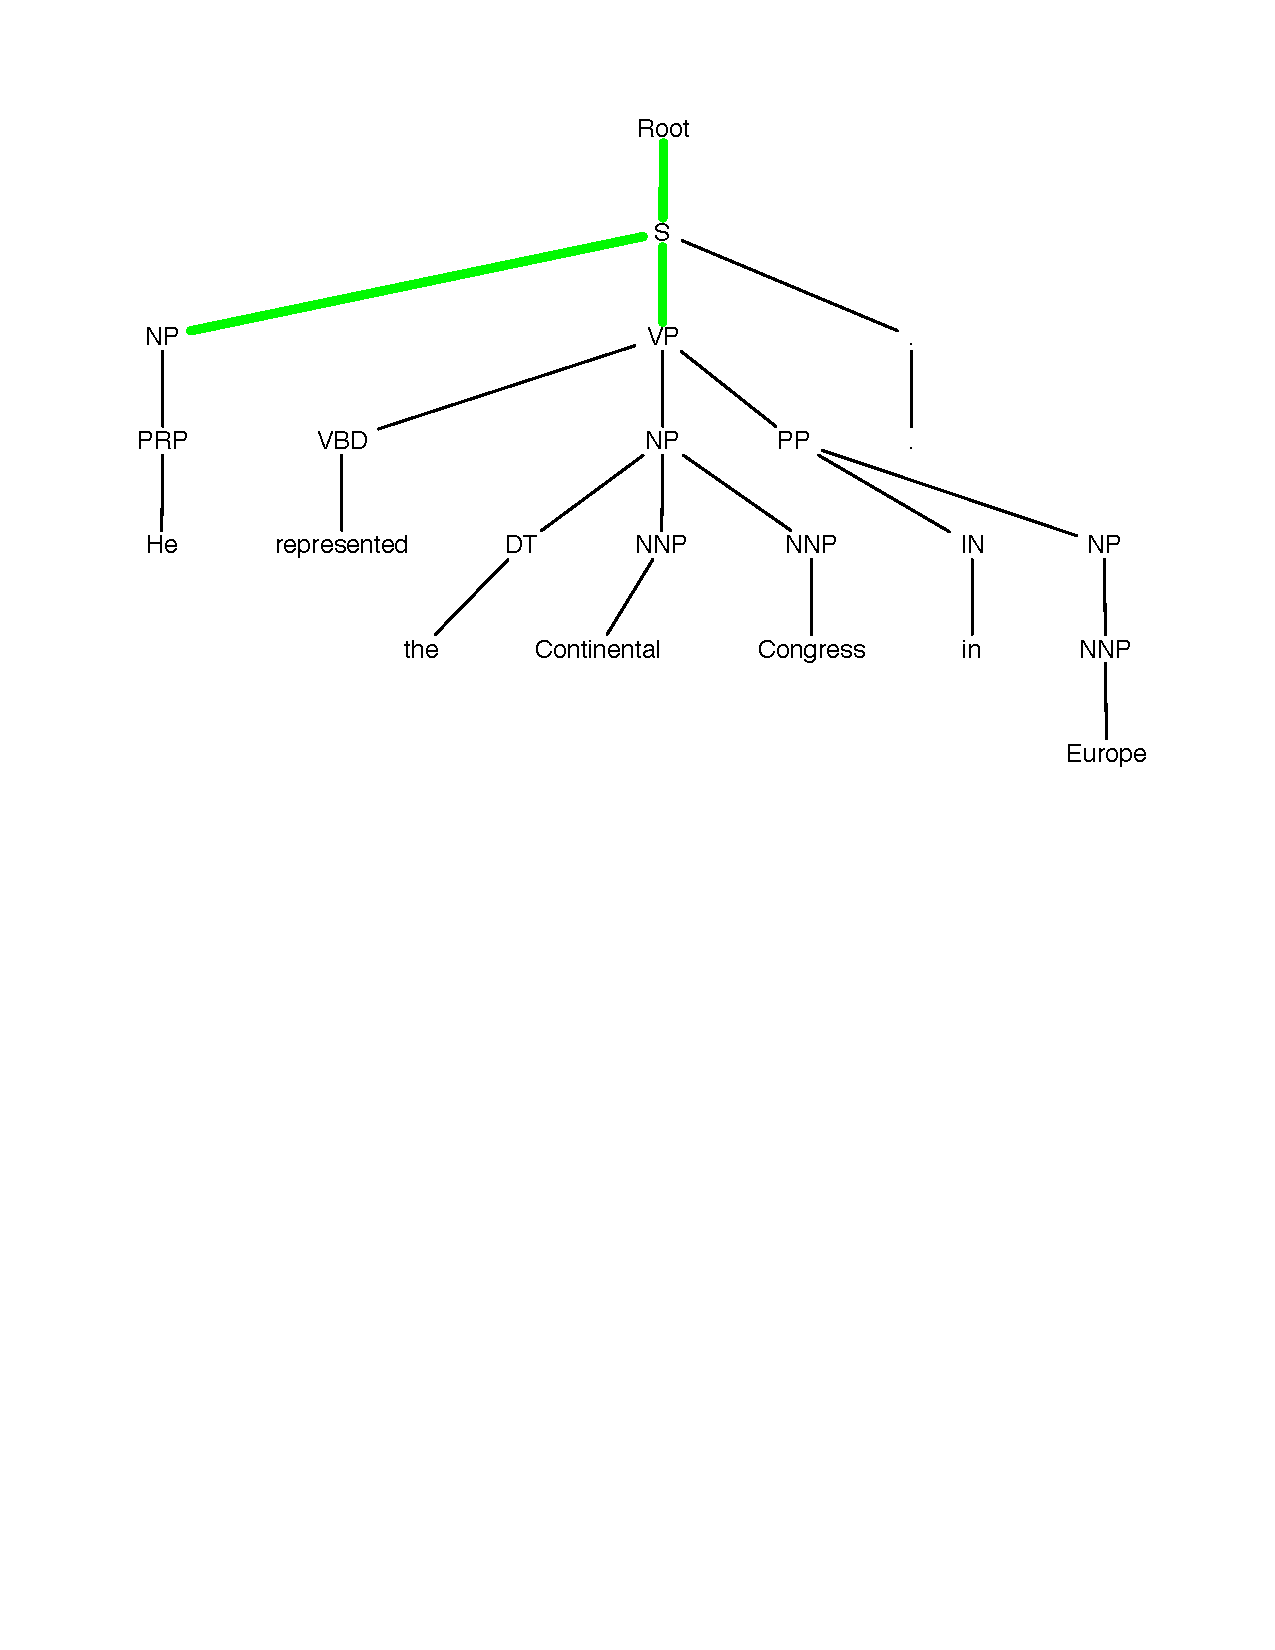
\includegraphics[scale=0.5]{factoid_matcher}
  
  \textsf{The green lines highlight the substructure searched for}
\end{center}

For example, this matcher will translate the sentence ``He achieved
international fame as the leading Union general in the American Civil War." into
the question ``Who achieved international fame as the leading Union general in
the American Civil War?''.

\subsubsection{DateMatcher}

\texttt{DateMatcher} is also derived from \texttt{ParseTreeMatcher}, but matches
trees of the form shown below. \texttt{DateMatcher} checks whether the given
parse tree has the substructure shown in the diagram and if the prepositional
phrase in the sentence contains a year (four consecutive digits was assumed to
be a year). To extract a question from such a sentence, the date is removed, and
``in what year?'' is appended.

\begin{center}
  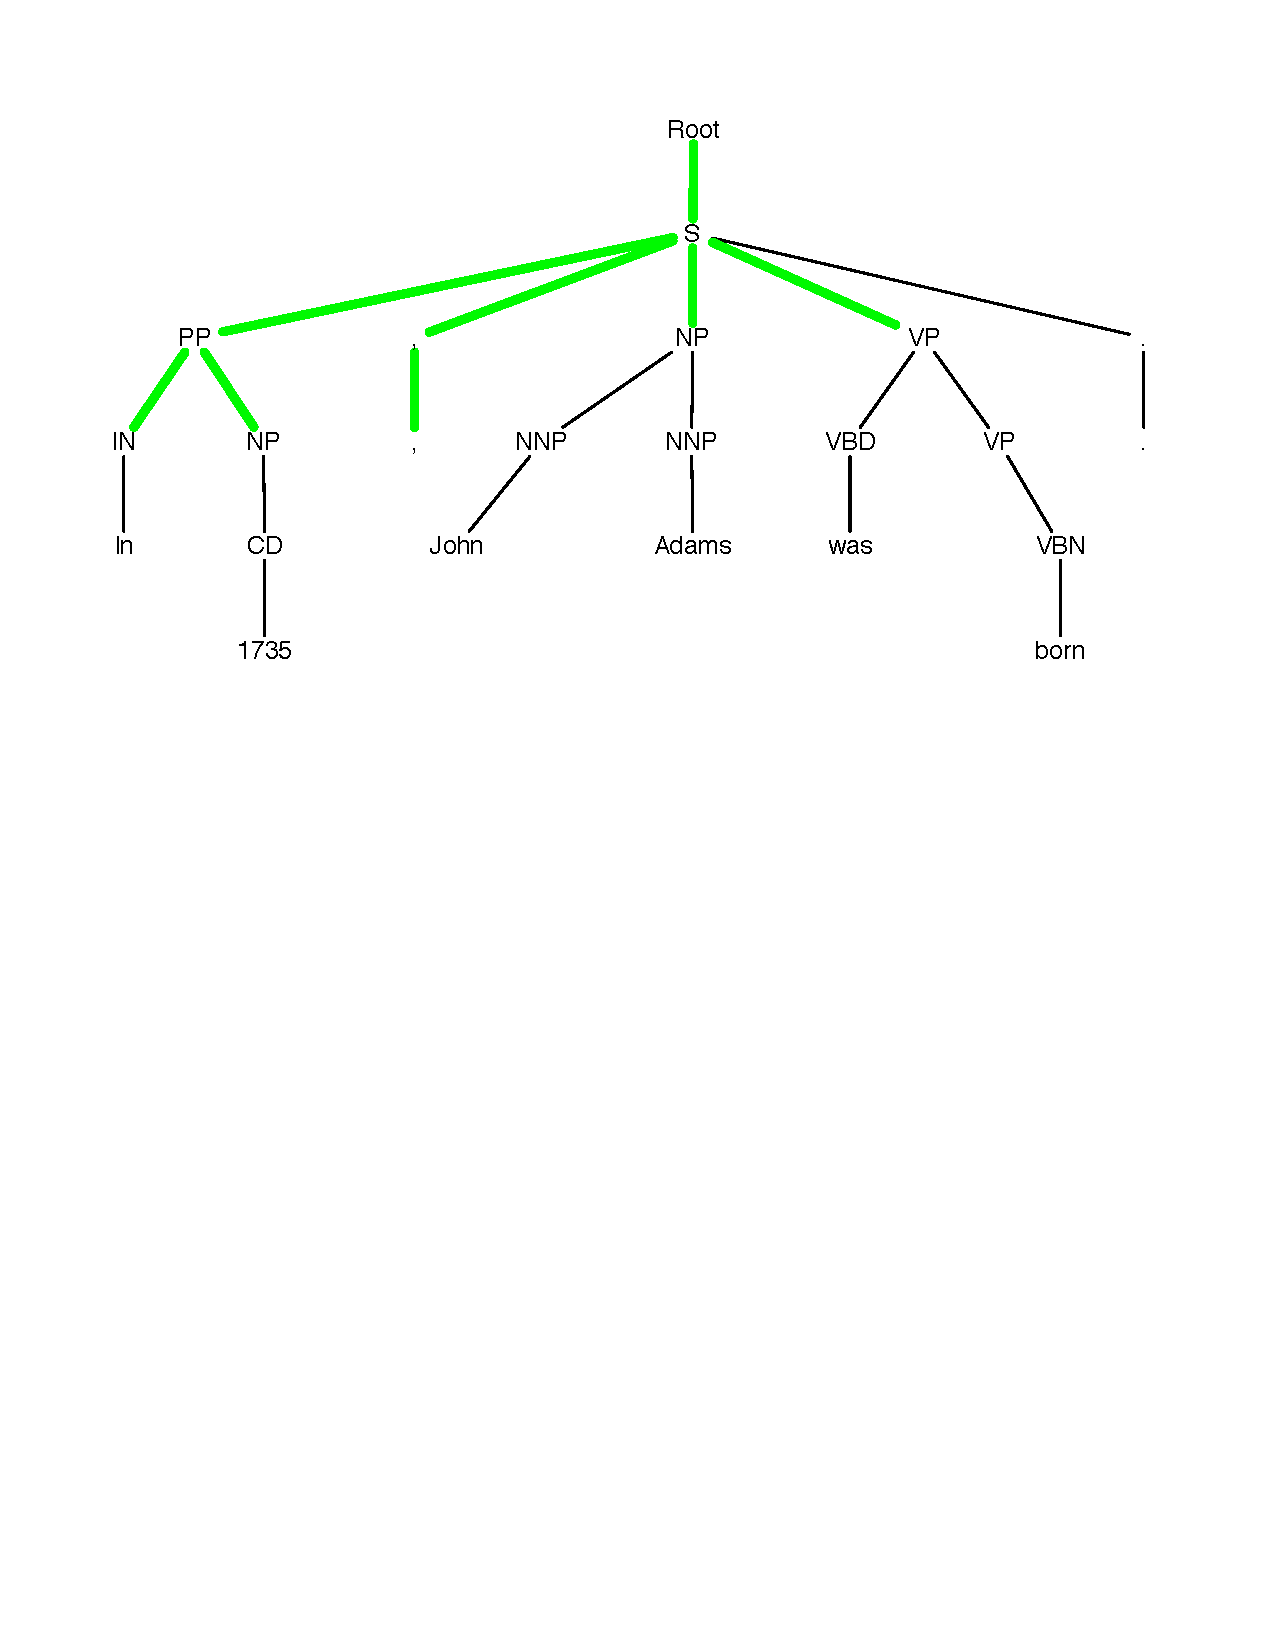
\includegraphics[scale=0.5]{date_matcher}
  
  \textsf{The green lines highlight the substructure searched for}
\end{center}

For example, this matcher will translate the sentence ``In 1860, he favored
Democrat Stephen A Douglas but did not vote.'' into the question: ``He favored
Democrat Stephen A Douglas but did not vote in what year?''

\subsection{Question Answering}
\subsubsection{answer}

\texttt{answer} takes the file name of the article and the file name of the
question file and returns a list of answers to the given questions. As with ask,
there is a verbose option for debugging. After reading in the article text,
answer reads in the questions one at a time and calls the \texttt{EasyAnswer}
module to extract answers.

\subsubsection{EasyAnswer}

Like \texttt{EasyQuestion}, the name of this component indicates that we
intended it to be used as a first solution to answering questions, falling back
to more sophisticated answering methods if this method proved insufficient.
However, this component is our only question-answering code, and we simply
print, ``Couldn't answer this question'' if it fails (i.e. not enough key words
from the question are matched in a sentence in the article.)

\texttt{EasyAnswer} takes a question and the full text of an article as input.
The key words of the question are extracted by stripping out common words and
removing punctuation, both tasks being implemented in the \texttt{CommonWords}
component. The remaining words are stemmed, and the resulting list of key words
is used for answer matching. The article title (always on the first line) is
removed from the key word list as well, to avoid false positives. After
separating the article text into sentences with \texttt{ArticlePreprocessor},
those too are stemmed to ensure consistency over the question and the article.
For each of the stemmed sentences, the number of keyword matches are counted and
the sentences are added to a list, keeping track of the sentence with the
highest score. If two sentences with the same score are found, the first matched
sentence has priority. After examining all the possible answers, if there are no
sentences that match at least half of the key words, the question is deemed
unanswered and \texttt{EasyAnswer} returns nil.

If there is a reasonable answer, we check whether the subject is a pronoun (if
it is, the first word will be the pronoun, so we only check the first word). If
the subject is ``it,'' the previous sentence is prepended so that the referent
will be included in the answer. While this is not guaranteed to include the
referent, very few coherent English sentences deal with referents further than
two sentences back so it will most likely work. If the subject is ``he'' or
``she,'' we substitute the article title; if it is ``they,'' the title is
pluralized and substituted. Finally, we capitalize the answering sentence
properly and return it.

\subsubsection{CommonWords}

\texttt{CommonWords} defines the words that we determined to be irrelevant to
finding the correct answer. Generally, these words fall into the categories of
determiners, auxiliary verbs, interogative pronouns, modals, prepositions, and
some conjunctions and adverbs. See the Appendix for a full list.

\texttt{CommonWords} has functions to remove common words from sentences, and to
strip trailing punctuation characters from single words (this is important in
question processing; there is always a ``?'' in a question, but it is never part
of a keyword).

\subsubsection{Stemmer}

The stemmer is an implementation of the Porter stemmer\footnote{\tt
http://tartarus.org/\~{}martin/PorterStemmer/} in Ruby by Ray Pereda. The module
Stemmable includes itself in the String class, so strings can call the function
stem. The calling string is stemmed then returned.

\subsubsection{Inflector}

The Inflector module is taken from the Active Support package (part of Ruby on
Rails). It contains (in \texttt{inflections.rb}) a variety of hard-coded rules
for pluralizing English words; we use this in the answering component, when
substituting the article title for the pronoun ``they''. See the Appendix for
details.

\section{Future Work}

The most significant aspect of the problem we struggled with was asking more
difficult questions. We had implementations in place to ask both medium
difficulty and hard questions, but ultimately removed them from our solution due
to coherency problems. These modules actually did make use of the ideas in our
initial plan; the medium difficulty questions were generated by extracting named
entities and adding ``what is'' or ``who is'' to them based on the categories to
form questions. The hard questions used a classifier to determine which of the
three article categories the given article belonged to and asked a series of
hard coded questions based on the category. If we had more time to deal with the
coherency problems, both would have been nice to include.

Our question asking solution was quite extensible, with its structure of
delegating the finding of good sentences and transforming them into answers to
the various ``Matcher'' components. We had some ideas for other matchers; for
example, one much like \texttt{FactoidMatcher} except that it would replace NPs other
than the subject NP with wh-words. We did not have time to implement these other
ideas.

An area we didn't explore and that would be significantly more work would be
implementing the question answering system that takes over when \texttt{EasyAnswer}
fails. \texttt{EasyAnswer} returns no answer if the best match sentence contains fewer
than half of the keywords, so there would be a need for a more advanced answerer
that deals with this case. Since our results were generally so good, we didn't
go in that direction, but it's a significant enough problem that if this
solution were to be released it would need to be dealt with.

\newpage

\begin{center}
  \Large{Appendix}
\end{center}

\noindent\large{\bf Common words}
\begin{verbatim}
  DETERMINERS = ['a', 'an', 'the', 'this', 'that', 'these', 'those']
  AUXILIARIES = ['be', 'am', 'is', 'are', 'were', 'was', 'been',
                 'do', 'does', 'did']
  WHWORDS = ['what', 'which', 'how', 'when', 'where', 'why', 'who']
  MODALS = ['will', 'can', 'may', 'might', 'would', 'should']
  PREPOSITIONS = ['of', 'in', 'for', 'with', 'at', 'from', 'to', 'as',
    'within', 'between', 'there', 'on', 'by']
  OTHERS = ['and', 'or', 'it', 'many', 'much']

  PUNCTUATION = ['?', '!', ',', '.', "'"]

  COMMONWORDS = [DETERMINERS, AUXILIARIES, WHWORDS, MODALS, PREPOSITIONS,
    OTHERS]
\end{verbatim}


\noindent\large{\bf Pluralization}

\noindent Each line adds a rule; input words are matched against the regex
in the first argument and, if they match, undergo the substitution in the
second argument. Words are matched starting with the last rule added.
\begin{verbatim}
  inflect.plural(/$/, 's')
  inflect.plural(/s$/i, 's')
  inflect.plural(/(ax|test)is$/i, '\1es')
  inflect.plural(/(octop|vir)us$/i, '\1i')
  inflect.plural(/(alias|status)$/i, '\1es')
  inflect.plural(/(bu)s$/i, '\1ses')
  inflect.plural(/(buffal|tomat)o$/i, '\1oes')
  inflect.plural(/([ti])um$/i, '\1a')
  inflect.plural(/sis$/i, 'ses')
  inflect.plural(/(?:([^f])fe|([lr])f)$/i, '\1\2ves')
  inflect.plural(/(hive)$/i, '\1s')
  inflect.plural(/([^aeiouy]|qu)y$/i, '\1ies')
  inflect.plural(/([^aeiouy]|qu)ies$/i, '\1y')
  inflect.plural(/(x|ch|ss|sh)$/i, '\1es')
  inflect.plural(/(matr|vert|ind)ix|ex$/i, '\1ices')
  inflect.plural(/([m|l])ouse$/i, '\1ice')
  inflect.plural(/^(ox)$/i, '\1en')
  inflect.plural(/(quiz)$/i, '\1zes')
\end{verbatim}

\end{document}